% 第6章
\section{評価と結果(\textcolor{green}{100\%})}
  \label{sec:評価と結果}
    \par
  
  \subsection{マッチングモデルの評価(\textcolor{green}{100\%})}
    \label{sec:マッチングモデルの評価}
      \par 本節では,これまでに開発したマッチングモデルの評価を行う.\ref{sec:数理最適化モデルの結果分析}項では,実データを用いたシミュレーションを実施し,その性能を分析する.\ref{sec:テストケースと結果}項では,テストケースによるモデルの妥当性の検証を行う.最後に,\ref{sec:複数モデルの比較検討}項にて,提案したモデルを他のモデルと比較し,その有用性を検討する.
  
      \subsubsection{数理最適化モデルの結果分析(\textcolor{green}{100\%})}
        \label{sec:数理最適化モデルの結果分析}
          \par 本項では,\ref{sec:数理最適化モデルの実装}節にて定式化及び実装を行った数理最適化ベースの割り当てモデルを用いて,実際のデータを用いたシミュレーションを行い,検証する.
          \par シミュレーションでは,タクシー・リムジン委員会(LTC)より提供されているニューヨーク市のタクシーのトリップデータ\scalebox{0.7}{\cite{YellowTaxiTripRecords}}を用いる.CtoCシェアサイクルサービスは今日までサービスとして提供されていないため,実運用されているデータを用いた検証を行うことは難しい.そのため,任意の2地点間を自由に移動できるという点で,ユーザの需要傾向に相関があると考え,タクシーの実運用データを利用することとした.シミュレーションを行う期間は2023年1月1日の0時から24時までの24時間である.この期間内に合計約7.7万のリクエスト数が存在している.自転車に関しては,ニューヨーク市内にランダムに10台配置した.検証上,簡単のため自転車台数は10台と少なくしている.
          \par シミュレーションを行う手順として,簡単な例を図とともに説明する.
          \par まず,図\ref{fig:割り当て前のユーザと自転車の初期状態}に示すように,ある任意の1分間に3人のユーザからの利用リクエストがストックされたとする.その際のユーザの位置を橙色のアイコンでプロットしている.また,その際の利用可能な自転車の配置状況も緑色のアイコンでプロットしている.これが割り当て処理を行う前のユーザと自転車の初期状態である.
          \par 次に,図\ref{fig:半径250mの自転車を対象とする制約}に示すように,制約条件を満たしているかどうかの確認を行う.ユーザから半径250m圏内に駐輪されている自転車のみを割り当ての対象としているため,その圏外に駐輪されている自転車はグレーアウトし,割り当ての対象として処理されない旨を表している.
          \par 図\ref{fig:ユーザの進行方向と自転者オーナの方向}では,割り当て処理のためのパラメータとなるユーザの進行方向と,自転車とその自転車オーナの方向を取得している.ユーザの場合,それぞれのユーザの現在地から目的地までを実線で表現している.自転車の場合,それぞれの自転車からその自転車のオーナの家までを破線で表現している.破線が表現されていない自転車は既にオーナの元に駐輪されていることを意味している.
          \par 最後に,割り当て処理を実施し,図\ref{fig:割り当て処理結果}に示すような割り当て結果となる.この図では,自転車とユーザの色は割り当て成功後のペアに対応している.数理最適化処理を行ったことによって,図中央にいるユーザには,半径250m圏内に自転車が駐輪されているものの,目的地方向がその自転車のオーナ方向との真逆であったことから割り当てられなかったことが分かる.
          \par そして,これと同様の処理を24時間分のトリップデータに対して行う.24時間の時間経過による自転車全体のステータスの変化を表した結果が図\ref{fig:自転車の割り当て成功率とステータスの変化}である.青色のグラフは,それぞれの1分間のリクエストストックに対して,どれくらいの割合で自転車が割り当てられたかを示している.緑色のグラフは,全体の自転車に対してどれくらいの自転車が現在利用中であるかを示している.赤色のグラフは,全ての自転車をオーナの元に戻す際の再配置コストを示しており,実態は,各自転車とオーナとの距離の総和で,自転車の散らばり具合を表す.

          \begin{figure}[htbp]
            \centering
            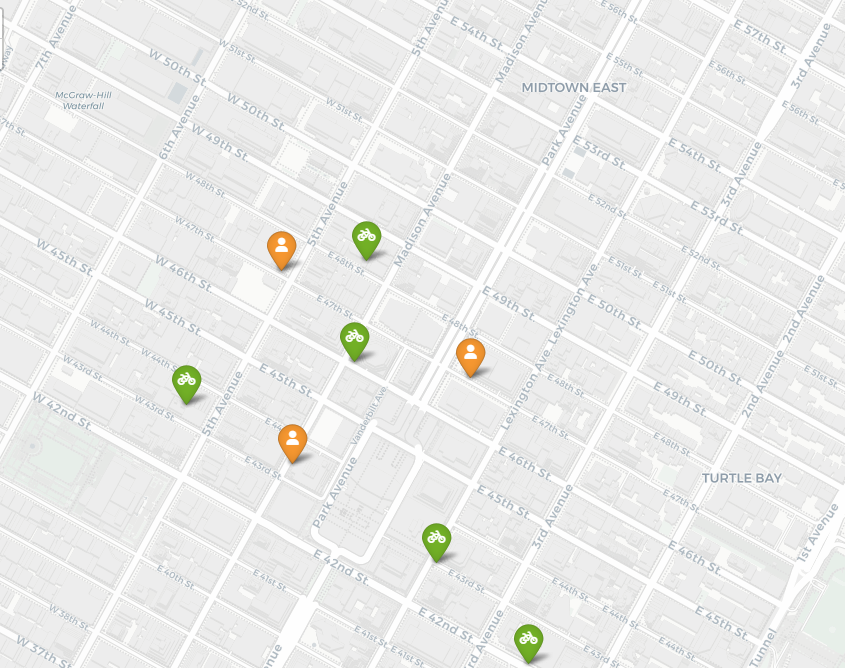
\includegraphics[scale=0.35]
            {figures/simulation1.png}
            \caption{割り当て前のユーザと自転車の初期状態}
            \label{fig:割り当て前のユーザと自転車の初期状態}
          \end{figure}

          \begin{figure}[htbp]
            \centering
            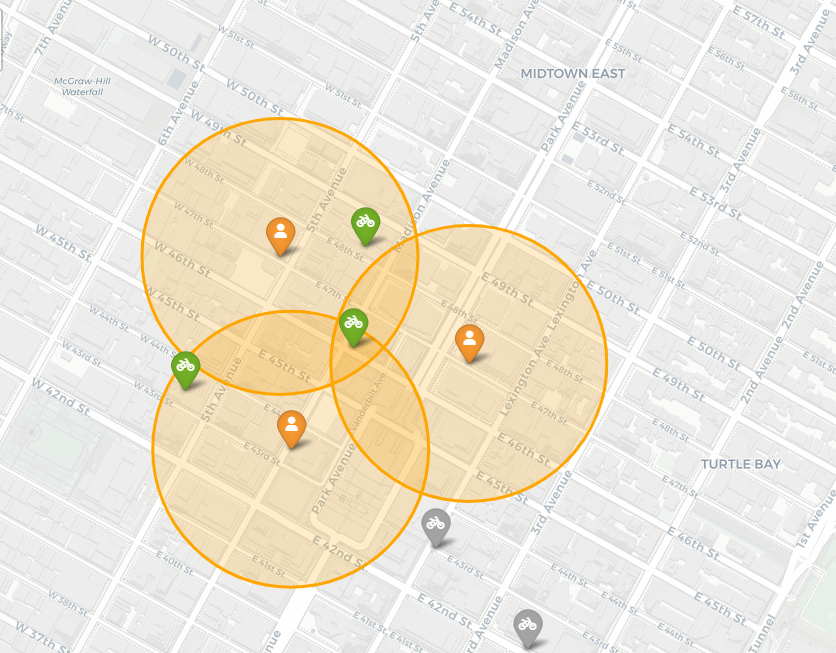
\includegraphics[scale=0.35]
            {figures/simulation2.png}
            \caption{半径250mの自転車を対象とする制約}
            \label{fig:半径250mの自転車を対象とする制約}
          \end{figure}

          \begin{figure}[htbp]
            \centering
            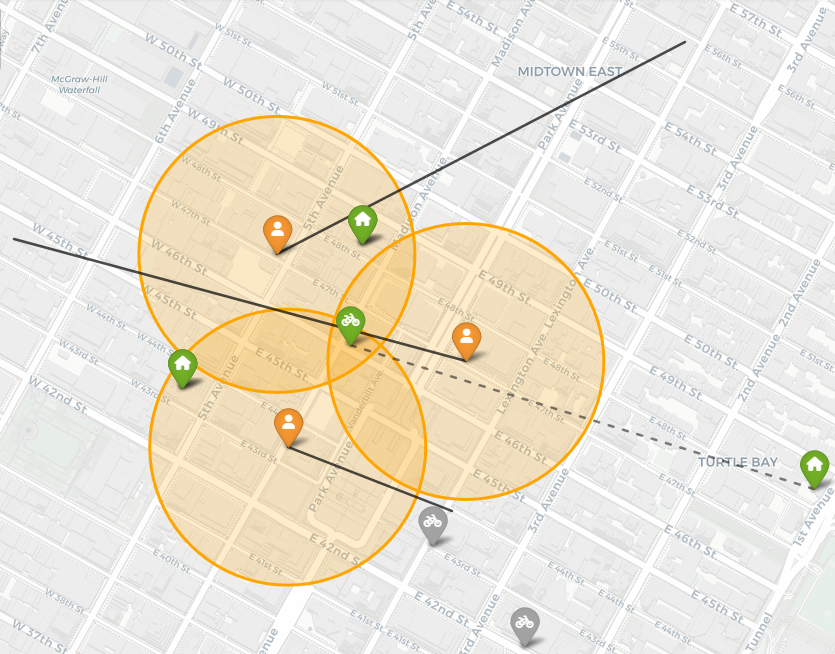
\includegraphics[scale=0.35]
            {figures/simulation3.png}
            \caption{ユーザの進行方向と自転者オーナの方向}
            \label{fig:ユーザの進行方向と自転者オーナの方向}
          \end{figure}

          \begin{figure}[htbp]
            \centering
            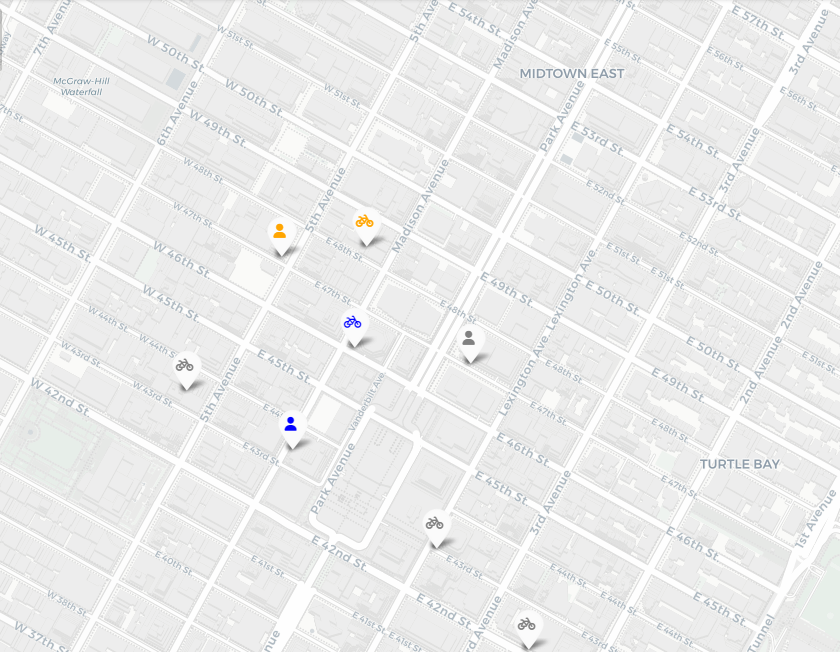
\includegraphics[scale=0.35]
            {figures/simulation4.png}
            \caption{割り当て処理結果}
            \label{fig:割り当て処理結果}
          \end{figure}

          \begin{figure}[htbp]
            \centering
            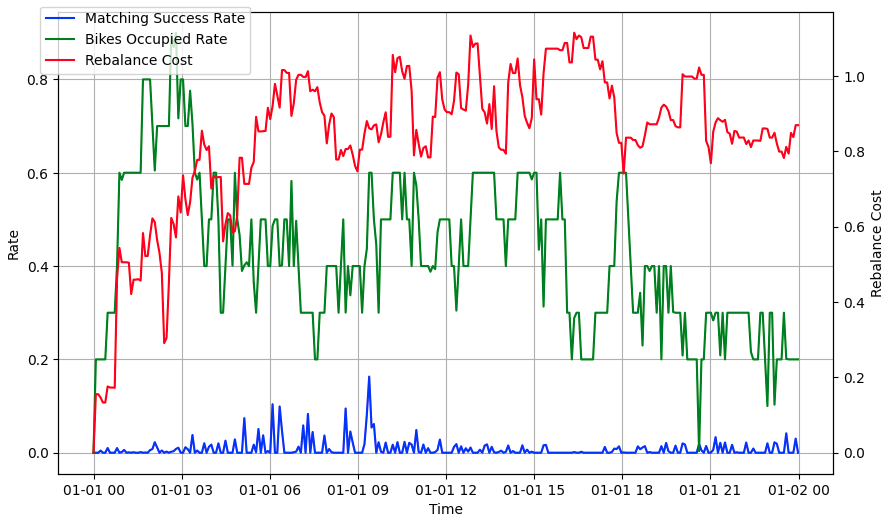
\includegraphics[scale=0.25]
            {figures/dispatchedResultFor1Day.png}
            \caption{自転車の割り当て成功率とステータスの変化}
            \label{fig:自転車の割り当て成功率とステータスの変化}
          \end{figure}

      \subsubsection{テストケースと結果(\textcolor{green}{100\%})}
        \label{sec:テストケースと結果}
          \par これまで,\ref{sec:数理最適化モデルの実装}節にてモデルの定式化やソルバーへの実装手順を示し,\ref{sec:数理最適化モデルの結果分析}項にて実際のデータを用いたシミュレーションを行った.本項では,それら実装したモデルやシミュレーションの妥当性の確認や解の品質評価を目的として,入力に対する出力の結果が意図する結果となっているかどうかを,テストケース及びテストコードを用意し,機械的に検証する.
          \par 数理最適化モデルが妥当な性能を発揮するかどうかを確かめるため,大きく分けて3種類のテストケースを用意する.それぞれ,小規模・中規模・大規模なデータである.小規模データでは,2台の利用可能な自転車が配置されている状態に対してユーザリクエストが1つ存在する状況のテストケースである.中規模データでは,5台の利用可能な自転車が配置されている状態に対してユーザリクエストが3つ存在する状況のテストケースである.大規模データでは,20台の利用可能な自転車が配置されている状態に対してユーザリクエストが10存在する状況のテストケースである.
          \par テストケースとして作成する自転車とユーザリクエストは,テスト観点を満たすための最低限のパラメータを持たせる.自転車は,現在地・自転車オーナの位置・利用終了予定時刻をパラメータとして持つ.ユーザリクエストは,利用開始位置・利用終了位置・利用開始時間・利用終了時間をパラメータとして持つ.また,\ref{sec:数理最適化モデルの結果分析}項のシミュレーションとは分離したテストを行うことでより妥当性が保証されるため,ニューヨークではなく東京周辺に自転車を配置したテストデータとする.
          \par 小規模データに関しては,さらに細かくテストケースを分割する.割り当てが成功する正常系と割り当てが失敗する異常系,制約条件を明らかに満たしていない例外ケースの3パターンを用意する.割り当てが失敗する異常系のテストケースは,表\ref{tab:小規模テストデータA及びBの自転車}及び表\ref{tab:小規模テストデータAのユーザリクエスト}に示す通りであり,これをテストデータAとしている.東京駅と新宿駅に2台の利用可能な自転車が駐輪されている状態で,東京駅から新宿駅までのユーザリクエストが存在しているシチュエーションである.結果としてユーザに自転車が割り当てられなかった.
          \par 割り当てが成功する正常系のテストケースは,表\ref{tab:小規模テストデータA及びBの自転車}及び表\ref{tab:小規模テストデータBのユーザリクエスト}に示す通りであり,これをテストデータBとしている.自転車の状態に関してはテストデータAに同じであるが,ユーザは,新宿駅から渋谷駅に向かいたいとする場合である.結果として新宿駅に駐輪されている自転車が割り当てられた.
          \par ここで,テストデータA及びBに関して,目的関数のパラメータを操作することによって,いかようにもなることが想定される.そのため,テストコード上で厳密に解の一致を判定することは行わず,想定しないエラーが発生せずに処理が完了することをテストしている.また,テストケースをカスタマイズして実際の挙動を確認する意義も果たしている.ただし,制約条件を明らかに満たしていない例外ケースはその限りではない.その場合はユーザに自転車が割り当てられるべきではないため,その旨が完全一致することをテストコード上で表現する.
          \par 具体的には,自転車の配置を表\ref{tab:小規模例外テストデータの自転車}に,ユーザリクエストは表\ref{tab:小規模テストデータAのユーザリクエスト}に示した通りのシチュエーションである.ユーザの利用開始位置に対して,自転車が明らかに制約条件を満たさない遠い距離に駐輪されている状態や,利用終了予定時間が未来である状態をテストしている.
          \par 小規模テストデータAやBと同じ要領で中規模データや大規模データに関してもテストケースを作成し,テストコードで機械的にテストを行えるよう整備した.データが大きくなるため,小規模データの説明の際に示したような表は割愛するが,付録のソースコードで確認できるため参照されたい.全てのテストケースに対して,それぞれ成功した場合は「SUCCESS」,失敗した場合は「FAILURE」をターミナルに出力できるようテストコードを整えて実行した結果が図\ref{fig:割り当てモデルのテスト}に示す通りである.全てのテストにパスしている.

          \begin{table*}[t]
            \caption{小規模テストデータA及びBの自転車}
            \label{tab:小規模テストデータA及びBの自転車}
            \centering
            \begin{tabular}{|l|l|l|l|} \hline
              自転車の現在地 & 自転車オーナの位置 & 利用終了予定時刻 & 場所(参考) \\ \hline
              (35.6804, 139.7690) & (35.6804, 139.7690) & NaT & 東京駅 \\
              (35.6895, 139.6917) & (35.6895, 139.6917) & NaT & 新宿駅 \\ \hline
            \end{tabular}
          \end{table*}
          
          \begin{table*}[t]
            \caption{小規模テストデータAのユーザリクエスト}
            \label{tab:小規模テストデータAのユーザリクエスト}
            \centering
            \begin{tabular}{|l|l|l|l|l|} \hline
              利用開始位置 & 利用終了位置 & 利用開始時間 & 利用終了時間 & 開始場所->終了場所(参考) \\ \hline
              (35.6804, 139.7692) & (35.6895, 139.6917) & now() & now()+15mins & 東京駅->新宿駅 \\ \hline
            \end{tabular}
          \end{table*}

          \begin{table*}[t]
            \caption{小規模テストデータBのユーザリクエスト}
            \label{tab:小規模テストデータBのユーザリクエスト}
            \centering
            \begin{tabular}{|l|l|l|l|l|} \hline
              利用開始位置 & 利用終了位置 & 利用開始時間 & 利用終了時間 & 開始場所->終了場所(参考) \\ \hline
              (35.6895, 139.6917) & (35.6618, 139.7012) & now() & now()+15mins & 新宿駅->渋谷駅 \\ \hline
            \end{tabular}
          \end{table*}

          \begin{table*}[t]
            \caption{小規模例外テストデータの自転車}
            \label{tab:小規模例外テストデータの自転車}
            \centering
            \begin{tabular}{|l|l|l|l|} \hline
              自転車の現在地 & 自転車オーナの位置 & 利用終了予定時刻 & 場所(参考) \\ \hline
              (35.8, 139.8) & (35.8, 139.8) & now()+1day & 足立区内某所 \\
              (35.81, 139.81) & (35.81, 139.81) & now()+1day & 埼玉県草加市某所 \\ \hline
            \end{tabular}
          \end{table*}

          \begin{figure}[htbp]
            \centering
            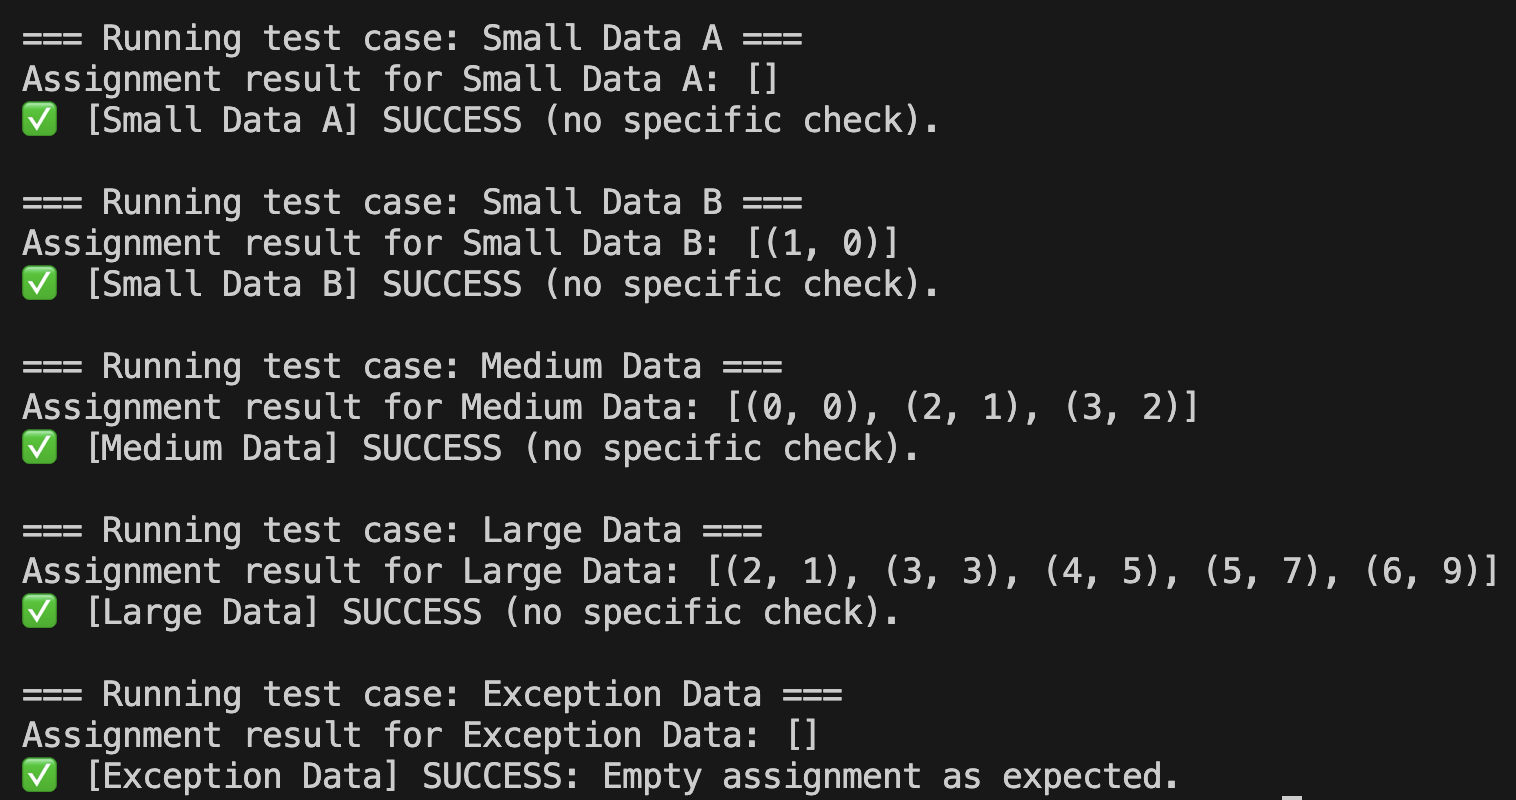
\includegraphics[scale=0.29]
            {figures/TestResult.png}
            \caption{割り当てモデルのテスト}
            \label{fig:割り当てモデルのテスト}
          \end{figure}

          
      \subsubsection{複数モデルの比較検討(\textcolor{green}{100\%})}
        \label{sec:複数モデルの比較検討}
          \par さらに,数理最適化モデルの有用性を検証するため,数理最適化モデルとは別の3つの割り当てモデルを構築し,比較検証を行う.構築する3つのモデルは,「ランダム割り当てモデル」「最近傍割り当てモデル」「逐次最適化割り当てモデル」である.
          \par ランダム割り当てモデルは,ユーザのリクエストに対してランダムに自転車を割り当てる.何の制約も存在しないため,現実的でない距離に駐輪されている自転車が割り当てられる可能性も十分にある.
          \par 最近傍割り当てモデルは,ユーザのリクエストに対して,そのユーザに最も近い位置に駐輪されている自転車を割り当てる.ユーザ視点からすると,最もユーザフレンドリな割り当てアルゴリズムである.
          \par 逐次最適化割り当てモデルは,ユーザのリクエストを1分間ストックすることなく,1リクエストに対して随時数理最適化割り当て処理を行う.これに伴い,本項内では通常の数理最適化モデルに対して「バッチ最適化割り当てモデル」と呼ぶこととする.
          \par それぞれのモデルに対して,\ref{sec:数理最適化モデルの結果分析}項にて行ったシミュレーション同様に,2023年1月1日の24時間のトリップデータを取り込み,自転車の割り当て処理を行う.
          \par 比較評価にあたって,それぞれのモデルを用いた場合の再配置コストを評価指標として選定する.本研究で提案してるCtoCシェアサイクルは,ドックレスで乗り捨てが可能であることを想定しており,その実現のためには,サービスを継続的に提供したとしても自転車が散らばらない状態が理想であるためである.その比較結果を図\ref{fig:モデル別再配置コストの時間経過比較}に示す.青色がランダム割り当てモデル,橙色が最近傍割り当てモデル,緑色が逐次最適化割り当てモデル,赤色がバッチ最適化割り当てモデルを表している.
          \par ランダム割り当てモデルと最近傍割り当てモデルは,サービス提供後ほどなくして再配置コストが上昇し,その後も高い値を推移している.
          \par 逐次最適化割り当てモデルは,サービス開始後8時間ほどはバッチ最適化割り当てモデルと同じような上昇トレンドであるが,8時間を超えたあたりからも再配置コストの上昇は継続され,最終的には,ランダム割り当てモデルや最近傍割り当てモデルと同等の再配置コストに収束した.結果としてバッチ最適化割り当てモデルの再配置コストが比較的低い値で推移することが分かった.
          \par さらに,どうようの比較を,ニューヨーク市内に自転車を50台ランダムに設置した場合でも行った.結果は\ref{fig:50台の時の再配置コストの時間経過比較}の通りである.傾向としては自転車を10台初期配置した場合と大差ないものの,よりその差が顕著に表れる結果となっている.

          \begin{figure}[htbp]
            \centering
            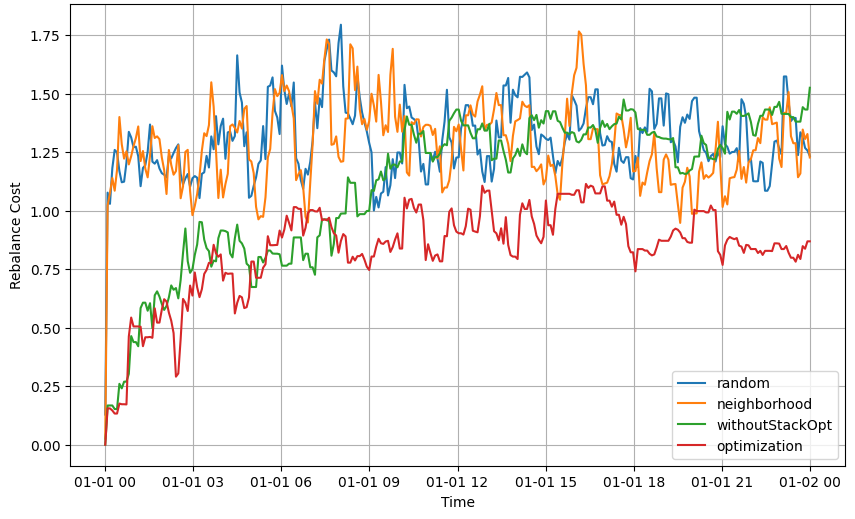
\includegraphics[scale=0.36]
            {figures/CompareRebalanceCost.png}
            \caption{モデル別再配置コストの時間経過比較}
            \label{fig:モデル別再配置コストの時間経過比較}
          \end{figure}

          \begin{figure}[htbp]
            \centering
            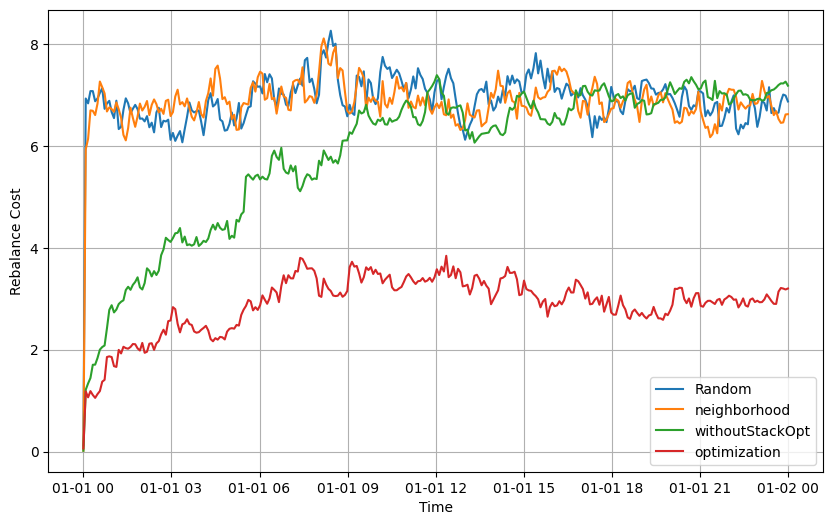
\includegraphics[scale=0.36]
            {figures/CompareRebalanceCost-50.png}
            \caption{50台の時の再配置コストの時間経過比較}
            \label{fig:50台の時の再配置コストの時間経過比較}
          \end{figure}
      
  % \subsection{APIの適用性評価(0\%)}
  %   \label{sec:APIの適用性評価}
  %     \par
      
  %     \subsubsection{都市への展開シミュレーション(0\%)}
  %       \label{sec:都市への展開シミュレーション}
  %         \par $\Box$ 統合テスト
  %         \par $\Box$ エンドツーエンド(E2E)テスト
          
  %     \subsubsection{スケーラビリティとパフォーマンス評価(0\%)}
  %       \label{sec:スケーラビリティとパフォーマンス評価}
  %         \par $\Box$ 負荷テスト
